\subsection*{Hypothesis 4}
Hypothesis 4 explores the impact of individual users' unique personalities, personal preferences,
and the potential for anonymous users to underrate books on rating scores.
We tested this hypothesis by considering the rating score as the primary metric and
any records with missing values were excluded from the analysis.
The hypotheses under examination were as follows:\\
\textbf{H0 (Null Hypothesis):} The rating score is not influenced by the user's profileName.
All rating scores are drawn from the same distribution, implying equal means and variances for each user's rating scores.\\
\textbf{H1 (Alternative Hypothesis):} The rating score is affected by the user,
suggesting that each user's rating scores follow a distinct distribution.\\
For the sake of consistency, users with fewer than 20 reviews were excluded from the analysis,
as a limited number of reviews cannot reliably estimate statistical measures.\\
The statistical test employed was ANOVA, which assesses differences in means between user groups.
The results yielded an F-statistic of 1.5374 and a corresponding P-value of 0.0670.
These results indicate that although there may be some variance in rating scores among different users,
the evidence to reject the null hypothesis (H0) and conclude that user personalities significantly impact
rating scores is not robust.\\
This conclusion is further supported by the accompanying boxplot (Figure \ref{fig:h4}),
which illustrates variations in the distribution of rating scores across users.
For what concerns the anonymous users, they do not seem to underrate books.
For what
\begin{figure}[H]
    \centering
    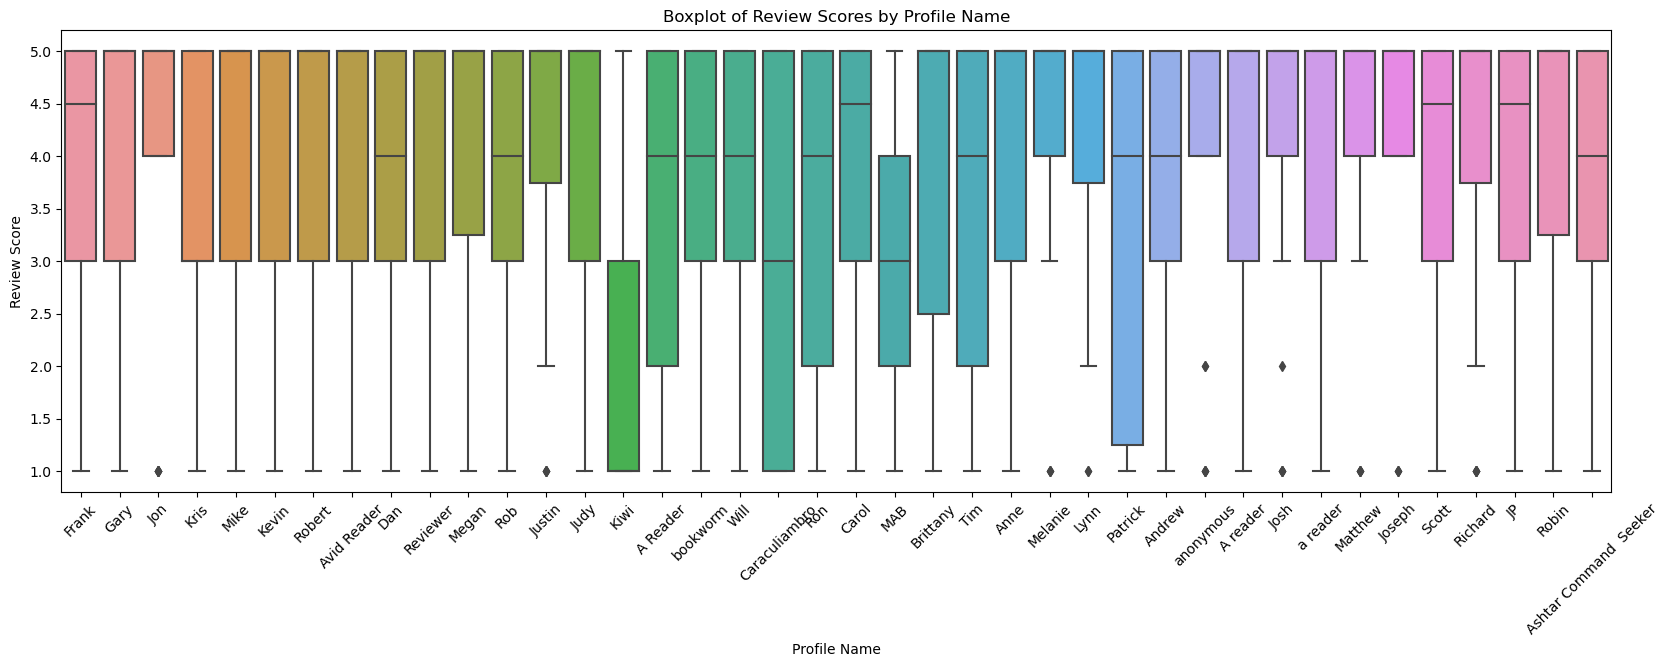
\includegraphics[width=0.5\textwidth]{./figures/h4.1.png}
    \caption{Distribution of rating scores across users}
    \label{fig:h4}
\end{figure}
